\documentclass[letterpaper,10pt,draftclsnofoot,onecolumn]{IEEEtran}
\usepackage{graphicx}
\usepackage{amssymb}
\usepackage{amsmath}
\usepackage{array}
\usepackage{amsthm}
\usepackage{listings}
\usepackage{alltt}
\usepackage{float}
\usepackage{color}
\usepackage{url}
\usepackage{setspace}
\usepackage{balance}
\usepackage{enumitem}
\usepackage{pstricks, pst-node}
\usepackage{inputenc}
\usepackage[margin=.75in]{geometry}

\lstset
{ %Formatting for code in appendix
    %frame=single,
    basicstyle=\footnotesize\ttfamily,
    numbers=left,
    numbersep=.25in,
    stepnumber=1,
    showstringspaces=false,
    tabsize=4,
    breakatwhitespace=false,
    xleftmargin=.5in,
    xrightmargin=.5in,
}

% JS options pulled from https://tex.stackexchange.com/questions/89574/language-option-supported-in-listings
\lstdefinelanguage{JavaScript}{
  keywords={typeof, new, true, false, catch, function, return, null, catch, switch, var, if, in, while, do, else, case, break},
  keywordstyle=\color{blue}\bfseries,
  ndkeywords={class, export, boolean, throw, implements, import, this},
  ndkeywordstyle=\color{darkgray}\bfseries,
  identifierstyle=\color{black},
  sensitive=false,
  comment=[l]{//},
  morecomment=[s]{/*}{*/},
  commentstyle=\color{purple}\ttfamily,
  stringstyle=\color{red}\ttfamily,
  morestring=[b]',
  morestring=[b]"
}

%crappy error with titlesec
\newcommand{\subparagraph}{}
\usepackage{titlesec}

\usepackage{fancyhdr}
\usepackage{hyperref}
\usepackage{tocloft}

%hide toc subsubsections
\setcounter{tocdepth}{2}
\setlength{\parindent}{.25in}

%toc formatting standards
\renewcommand{\cftsecleader}{\cftdotfill{\cftdotsep}{\vspace{.25cm}}}
\renewcommand{\cftsecfont}{\normalfont}
\renewcommand{\cftsecpagefont}{\normalfont}
\renewcommand{\cftsecaftersnum}{.}

%bottom right page numbers
\fancyhf{}
\renewcommand{\headrulewidth}{0pt}
\rfoot{\thepage}
\pagestyle{fancy}

%formatting Section headings
\titleformat{\section}[block]
  {\fontsize{12}{12}\bfseries\sffamily}
  {\thesection.}
  {1em}
  {\vspace{.1cm}}
\titleformat{\subsection}[block]
  {\fontsize{12}{15}\slshape\sffamily}
  {\thesubsection}
  {1em}
  {\vspace{.1cm}}
\titleformat{\subsubsection}[block]
  {\fontsize{11}{20}\slshape\sffamily}
  {\thesubsubsection}
  {1em}
  {\vspace{.1cm}}
  
\geometry{textheight=8.5in, textwidth=6in}

\renewcommand{\thesection}{\arabic{section}}
\renewcommand{\thesubsection}{\thesection.\arabic{subsection}}
\renewcommand{\thesubsubsection}{\thesubsection.\arabic{subsubsection}}

\newcommand{\cred}[1]{{\color{red}#1}}
\newcommand{\cblue}[1]{{\color{blue}#1}}

\def\name{Charles Siebert}

%% The following metadata will show up in the PDF properties
\hypersetup{
  urlcolor = black,
  pdfauthor = {\name},
  pdfkeywords = {cs462 ``Senior Capstone - Spring 2017'' capstone},
  pdftitle = {CS 462 Progress Report - Spring 2017},
  pdfsubject = {Capstone Progress Report - Spring 2017},
  pdfpagemode = UseNone
}

\begin{document}
\begin{titlepage}
\centering
\vspace*{6cm}
{\scshape\LARGE \begin{singlespace}Optimizing Virtual Reality and Augmented Reality Performance on Mobile Web Applications \\ \end{singlespace} \smallskip Group 52 - Progress Report } \\
	{\scshape\Large CS462 - Spring 2017 \par}
	\vspace{.5cm}
	\name \par
    {\large May 15, 2017 \par} 
	\vspace*{1cm}
	
\begin{abstract}
The technology of Virtual Reality (VR) currently is not cost effective to today's market, as the cost of high-end setups required makes it difficult to afford. Browser developers are focusing primarily on expensive high-end high-performance hardware over mobile devices for Augmented Reality (AR) or Virtual Reality (VR) on the web. Doing AR/VR on the mobile web allows more developers to enter the field and deliver to more customers. To accomplish this, we are working on a project called �Mobile AR/VR Performance�, which focuses on researching to profile and identify performance bottlenecks in 3D web content on mobile devices. We will file issues in the open source projects for Chrome, Firefox through A-Frame and Three.js to determine and identify those bottlenecks. We hope to accomplish this by reporting the challenges and opportunities for performance VR/AR applications, and write a blog post detailing the project results and their best-practices.
\end{abstract}

\end{titlepage}

\newpage

\thispagestyle{empty}
\pagenumbering{gobble}

\tableofcontents

\cleardoublepage
\pagenumbering{arabic}

\newpage

\begin{singlespace}

\section{Purpose and Goals}
This paper is a progress report for group 52, "OVRAR" over the past 6 weeks for the Spring Term for 2017. Our group has finished the development for our project and has pushed out our results to our client in the form a blog post to their industry research site.

The purpose of this project is to determine areas of development within A-Frame where practices will be best used, as they will least be likely to impede on bottle necking either the software or hardware when optimizing the software for performance. This project is focused towards the advancement of an open-source, developing web framework, and the developers making their own products with A-Frame and for mobile devices. The developers will be using our project research as a means to avoid these bottlenecks in this evolving environment. Developers other than us will use the information in the report to determine the best way to approach at designing their programs, as the software we create will only serve as test cases and stress testing for mobile devices to collect this information.

Optimizing VR and AR for Mobile Web Apps is to determine Virtual Reality (VR) and Augmented Reality (AR) bottlenecks that exist in mobile devices within the A-Frame framework. The bottlenecks can be caused from either unoptimized development of software, underpowered or unoptimized hardware found in existing devices, or potential bugs or limitations found within the framework itself. The software itself, which is developed on A-Frame, will generate multiple scenes where it will test the graphical capabilities of the hardware within the mobile devices, the types of different implementations of certain scenes, and determine areas of optimization through these multiple scenes. The software will be used to create a report that will analyze the information collected about processing power, frame rates, battery usage, and the limitations of the framework to determine the best practices for implementing more graphically intensive programs on A-Frame.

\section{Group Reports}
Over the past 6 weeks, each of us has submitted weekly updates to describe the progress over the past week, the problems we encountered during the week, and the plans we have for the next week. This is to keep track of our progress as we move through the project time-line, and determine whether we are on track, or behind our current schedule.

\subsection{Charles Siebert}
The following sections include weekly summaries and a retrospective reflection over the past 6 weeks for Charles Siebert.

\subsubsection{Weekly Summaries}

\subsection{Branden Berlin}
The following sections include weekly summaries and a retrospective reflection over the past 6 weeks for Branden Berlin.
	
\subsubsection{Weekly Summaries}

\subsection{Yipeng "Roger" Song}
The following sections include weekly summaries and a retrospective reflection over the past 6 weeks for Yipeng "Roger" Song.

\subsubsection{Weekly Summaries}

\subsection{Interesting Code Snippets}

During our development, one of our testing cases was to test the lighting calculations that would be based off the normal vectors on each face being rendered in our geometries. We realize this would cause an impact the more calculations it would be doing (i.e. denser polygon objects, and number of lights). We created lights to be turned on individually by the user as soon as the cursor enters the object. This allows us to determine the performance impact on each light being turned on, one at a time, illuminating the test objects we have picked out. The following code snippet attached a light, and an event listener to an object we render to the screen, allowing the user to hover over the object to perform whatever action we tie to it, and in this case, increase the lighting intensity.

\begin{lstlisting}[language=JavaScript]
var radius = 10;
var entityBall = document.createElement('a-sphere');
entityBall.setAttribute('scale', {
	x: 2,
	y: 2,
	z: 2
});
entityBall.setAttribute('position', {
	x: radius * Math.cos(1/10 * 2 * Math.PI),
	y: 3.8,
	z: radius * Math.sin(1/10 * 2 * Math.PI),
	radius: 10
});                                      
entityBall.setAttribute('light', {
    type: 'point',
    color: '#424242',
	intensity: .1,
	decay: 1
});
entityBall.addEventListener("mouseenter", function(d,i) {
	entityBall.setAttribute('light', {
	color: '#ffffff',
	intensity: 1,						
	});
})
sceneEl.appendChild(entityBall);
\end{lstlisting}

\subsection{Draft Blog Write-up}
As a section of the blog post we wrote up for Mozilla contains a lot of introductory information already presented in this document, we will cut to the relevant information that provides our research approach towards our test cases and discuss the results.

Ultimately, we wanted to break up the aspects of rendering computer graphics onto the screen to determine the performance impact they would individually have on our Nexus 5X. As we took the approach of first implementing for optimized performance, we created standards of performance that the phone should be pushing. For a VR experience, having smooth frame rates is a priority for a proper usability experience. Our first round of implementations allowed us to reach a baseline 30 FPS in most of our rooms.Our second round of implementation is used to find the upper bounds of the limits of A-Frame. We found that we can remove the limits we imposed on ourselves in all of the previous rooms and attempt to see if we can cause anything to break, or find something unsupported. Since we wanted to test specific aspects of graphics rendering within A-Frame. We created a VR environment in which a user can select from eight rooms to see a completely different scene, all testing different components, such as object modeling, texturing, animations, and lighting.

To see the performance impact by finding the upper bounds, we implemented a higher resolution tree in our second round of implementation. To see the performance impact, of loading large amount of low vertice count objects compared to a low amount of high vertice count objects. By having a comparable amount of vertices being rendered in either scene will help us determine the performance impact on loading multiple objects at once through our assets. In the second room, we also implemented high resolution textures to compare the performance impact on loading the assets directly from the website based on the file sizes of each texture. The third room, we looked into the impact on lighting the low-poly trees compared to the high-poly trees when a new light is turned on during rendering. Our team realized that any developers looking at our testing isn�t only going to implement just models with no lighting, or just a room full of animated objects. The fourth room implements all of the features together to simulate what an actual developer might create.

After finishing our benchmark development, our team found a couple of interesting results from our testing. Resizing textures to a power of two heavily increases the workload on loading and rendering the scenes. Since the framework resizes it to the nearest power of two, we found that high-resolution textures that didn�t match the criteria and reached sizes of 8196x8196, and one texture taking up to 20 MB. We found with this implementation, that having upwards 70 MB of assets to be loaded for one web page to be unrealistic in a phone environment, as well as causing significant delays in loading the scene properly, and in some cases, crashing Firefox Beta (v.54.0) on our phones.

We also found that our higher resolution trees further causes delays in in loading the models, and significant slowdowns in rendering the scenes. Our high resolution tree features 37,000 vertices which increases the amount of workload the graphics has to render, including lighting from multiple light sources. This heavily limited the amount of models we could load into our scene. We also found an upper limit for our devices with handling these trees, and when our room reached about 1,000,000 vertices, our phone browsers would crash after a couple of minutes of attempting to load and render.

We found a linear increase in load times based off of the amount of models to be drawn to the scene. Having hundreds of models drawn to the scene added to be a significant amount of time if each object to be loaded took, for example, three milliseconds. Further inspecting the memory snapshot shows that our object models are read in and stored into object arrays for quicker access and rendering. Larger object models would also increase linearly based off the amount of vertices and faces are used to create the model, and their resulting normal vectors.

During the testing while using WebIDE to monitor and grab the performance data, we found that the extra overhead of USB Debugging on our Android devices caused our performance to drop by nearly half. Our testing showed that CPU Performance was not the leading bottleneck in rendering the scenes. In Figure 1, it shows that the CPU Usage was hovering at 10-25\%, while still experiencing heavy performance drops. This shows that the rendering is mostly done on the GPU, which follows suit with how OpenGL ES 2.0 operates, which is what this framework utilizes.

\section{OVRAR's Development Pictures}

\begin{center}
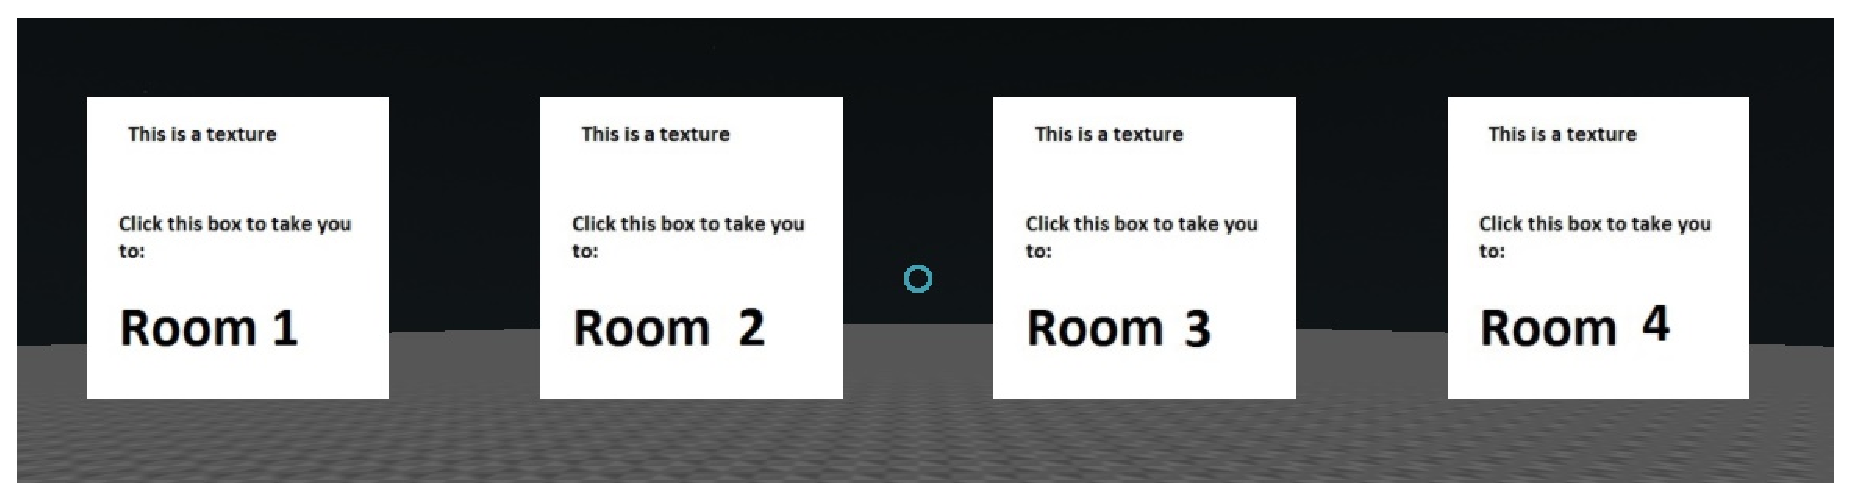
\includegraphics[width=\textwidth]{lobby.eps}\\
\textbf{Figure 1. } The lobby with eight traversal links to new rooms.\\
\vspace{.75cm}
\includegraphics[width=\textwidth]{room1r.eps}\\
\textbf{Figure 2. } Room 1r with multiple trees scattered in the scene.\\
\vspace{.75cm}
\includegraphics[width=\textwidth]{room2r.eps}\\
\textbf{Figure 3. } Room 2r demonstrating some animations (it actually is animated).\\
\vspace{.75cm}
\includegraphics[width=\textwidth]{room3r.eps}\\
\textbf{Figure 4. } Room 3r has some specific user interactions when hovering over the spheres. \\
\vspace{.75cm}
\includegraphics[width=\textwidth]{room4r.eps}\\
\textbf{Figure 4. } Room 4r combines all aspect to put together an interesting scene. \\
\vspace{.75cm}
\end{center}

\end{singlespace}

\end{document}

